\section{Introduction}\label{sec:Introduction}

%%%%%%%%%%%%%%%%%%%%%%%%%%%%%%%%%%%%%%%%%%%%%%%%%%%%%%%%%%%%%%%%%%%%%%%%%%%%%%%%%
\subsection{Importance of drift velocity and electrict field determination}\label{sec:Intro}
%%%%%%%%%%%%%%%%%%%%%%%%%%%%%%%%%%%%%%%%%%%%%%%%%%%%%%%%%%%%%%%%%%%%%%%%%%%%%%%%%
Some reason why this is important.


%%%%%%%%%%%%%%%%%%%%%%%%%%%%%%%%%%%%%%%%%%%%%%%%%%%%%%%%%%%%%%%%%%%%%%%%%%%%%%%%%
\subsection{Setup description and important definitions }\label{sec:Def}
%%%%%%%%%%%%%%%%%%%%%%%%%%%%%%%%%%%%%%%%%%%%%%%%%%%%%%%%%%%%%%%%%%%%%%%%%%%%%%%%%
LArIAT has 3 drift volumes: a main one between cathode and shield plane, and two smaller ones between shield and induciton planes (SI) and between induction and collection planes (IC). Scope of this work is to measure the drift velocity and electric field in the main drift volume using data.

For the data considered, we assume the voltages applied on shield, induction and collection planes are known and constants. Their value can be found in table \ref{tab:voltages}.
For RunI and RunII data, the spacing between both the shield and induction planes and the induction and collection planes is 4 mm. 

Table \ref{tab:Efields} reports the values of the electric field, drift velocity and drift times; the next few paragraphs describe how these quantities are calculated.  The electric field is calculated using equation \ref{eq:Efield}:

\begin{equation} E_{field}=\frac{\Delta V_{ab}}{\Delta x}, \label{eq:Efield}
\end{equation}
where $\Delta V_{ab}$ is the voltage difference between two consecutive anode planes and $\Delta x$ is their spacing.

\begin{table}[]
\centering
\caption{Anode planes voltages}
\label{tab:voltages}
\begin{tabular}{lll}
\hline
\multicolumn{1}{|l|}{VShield} & \multicolumn{1}{l|}{VInduction} & \multicolumn{1}{l|}{VCollection} \\ \hline
\multicolumn{1}{|l|}{-298.75} & \multicolumn{1}{l|}{-18.5}      & \multicolumn{1}{l|}{338.5}       \\ \hline
                              &                                 &                                 
\end{tabular}
\end{table}



 
\begin{table}[]
\centering
\caption{Electric field and drift velocities in LArIAT smaller drift volumes}
\label{tab:Efields}
\begin{tabular}{|l|l|l|}
\hline
& Shield-Induction & Induction-Collection \\ \hline
E$_{filed}$ &                 700.625 V/cm        &                892.5  V/cm             \\ \hline
v$_{drift}$ &                   1.70  mm/$\mu$s   &                  1.86 mm/$\mu$s        \\ \hline
t$_{drift}$ &                   2.35  $\mu$s      &                   2.15 $\mu$s           \\ \hline

\end{tabular}
\end{table}

From the electric field, we calculate the drift velocity and substquently the drit time in the volumes bewteen shield and induction planes and induction and collection planes.
The relationship between drift time and drift velocity is straightforward ($v_{drift} = \Delta x/t_{drift}$), but the one between  electric field and drift velocity is more complicated. The relationship between the electric field and drift velocity in LAr can be described as 
\begin{equation} v_{d} = \mu(E_{field},T) E_{field}, \label{eq:vd}
\end{equation}
where where $\mu$ is the electron mobility in LAr and T the temperature. The electron mobility depends on the LAr temperature and the electric field. The empitical formula for this dependency is described in ~\cite{WWW} and shown in figure \ref{fig:EV} for several argon temperatures.


\begin{figure}[ht!]
\centering
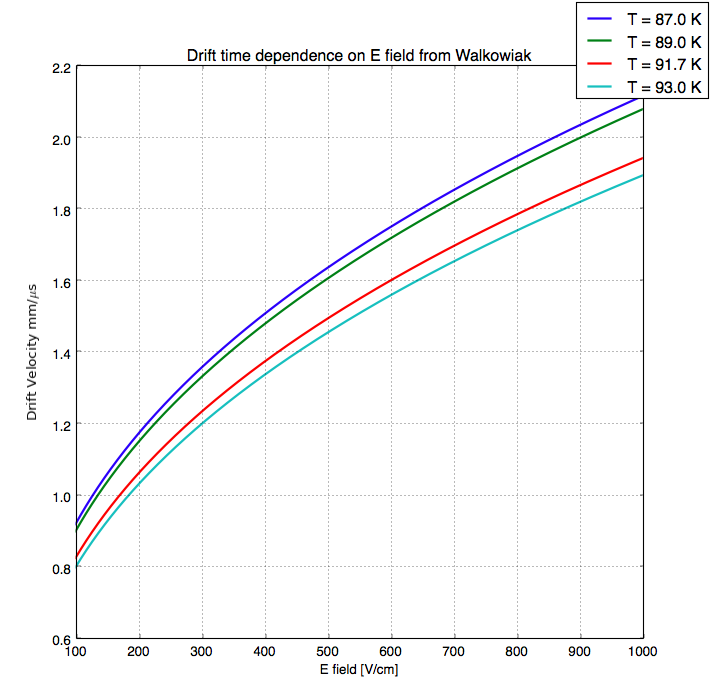
\includegraphics[scale=0.45]{./images/Walkowiak.png}\\
\caption{Drift velocity dependence on electric field for several temperatures.}
\label{fig:EV}
\end{figure}


In order to determine the temperature inside the TPC, we read the measure from the S651PDZ36A thermal ribbon RTDs in ACNET. 
LArIAT is equipped with three temperature probres inside the LAr: one at the bottom (TE213A in figure \ref{fig:cryo}), one in the middle (TE314A in figure \ref{fig:cryo}) and one on the top of the cryostat (TE212A in figure \ref{fig:cryo}). In what follows, we assume the reading of the middle probe is a good estimated of the temperature inside the whole TPC. Thus, we assume the temperature to be 91.7K. \textcolor{red}{On average}, the three probes read as shown in table \ref{tab:temp}. 
\begin{table}[]
\centering
\caption{Average temperatures measured at the top, middle and bottom in the LArIAT cryostat.}
\label{tab:temp}
\begin{tabular}{|c|c|c|}
\hline
Top Probe Temp (TE212A) & Middle Probe Temp (TE214A)   & Bottom Probe Temp (TE213A)  \\ \hline
91.7 $\pm$ 0.7 K &  91.8 $\pm$ 0.7 K                   & 93.3 $\pm$ 2.7 K       \\ \hline
\end{tabular}
\end{table}


\begin{figure}[ht!]
\centering
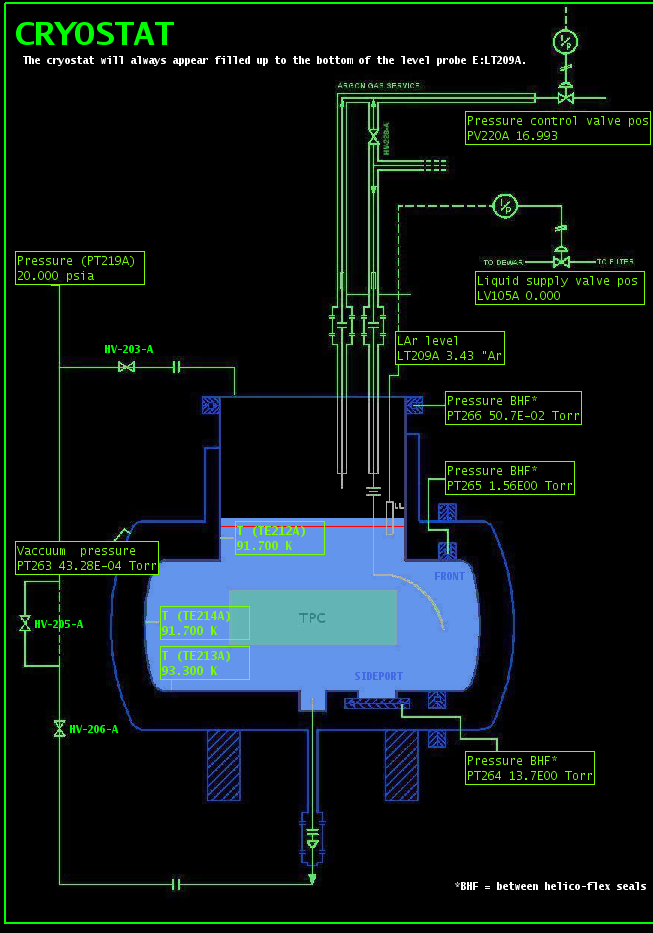
\includegraphics[scale=0.45]{./images/cryopic.png}\\
\caption{Scheme of LArIAT cryostat and cryo probes.}
\label{fig:cryo}
\end{figure}


As a cross check, it can be noted that the pressure in the cryostat is maintained constant at 20 psi at the liquid argon surface (PT219A in figure \ref{fig:cryo}), which corresponds to argon temperature of  90.328K,  according to NIST RefProp [\textcolor{red}{reference}]. In oder to calculate the pressure (and subsequently the temperature) in the middle of the TPC, we consider about 40 cm of Argon from the lulage surface. This argon raises the pressure of about 0.79 psi. A pressure of ~20.79 psi corresponds to a temperature to ~90.8 K according to NIST.  So, ball park!

  

\clearpage
\newpage
\section{Methodologies}\label{sec:Methodologies}
This section describes three different methodologies to measure the electric field in the LArIAT main drift volume.  
\subsection{E field using electrical diagram}\label{sec:elDiagram}
The electric field in the LArIAT main drift volume can be determined knowing the voltage applied to the cathode, the voltage applied at the shield plane and the distance between them. We assume the distance between the cathode and the shield plane to be 470 mm and the voltage applied to the shield plane to be -298.75 V. The only quantity left to dermine is then the voltage applied at the cathode. We can derive this latest quantity by using ohm's laws on the ciruit shown in fig \ref{fig:circuit}. We want to calculate the voltage at point B with respect to ground (point C). From ACNET readings, the volatge provided by the power supply is 23.5 kV and the glasmsman current reading is 0.0417 $\pm$ 0.015 mA (see figure \ref{fig:currentMeasurement}). LArIAT is equipped with two 40 $M\Omega$ filter pots in series, which correspond to an equivalent resistor of 80 $M\Omega$. Thus, the voltage at the cathode is:

\begin{equation} V_{BC}=V_{PS} - I*R_{eq} = -23.5kV + 0.0417mA*80M\Omega = -20.162 kV, \label{eq:Efield}
\end{equation}
where I is the current and R$_{eq}$ is the equivalent resistor.
The electric field, drift voltage and drift time are then calculated to be

\begin{equation}E_{filed} = \frac{V_{BC} - V_{shield}}{\Delta x} = 422.63 \textit{ V/cm} 
\end{equation}
\begin{equation}v_{drift} = \mu E_{field} = 1.403 \textit{ mm/$\mu$s}
\end{equation}
\begin{equation}t_{drift} = \frac{\Delta x}{v_{drift}} = 3349.29 \textit{ $\mu$s.}
\end{equation}

\begin{figure}[hp]
\centering
\begin{minipage}{0.45\textwidth}
\centering
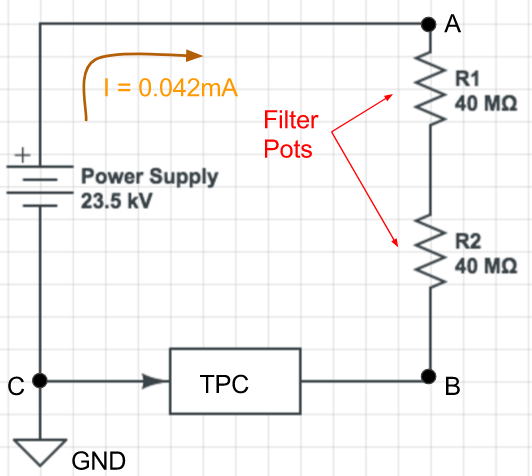
\includegraphics[width=3in]{images/CircuitLArIAT.png}
\caption{LArIAT HV simple schematics.}
\label{fig:circuit}
\end{minipage}\hfill
\begin{minipage}{0.45\textwidth}
\centering
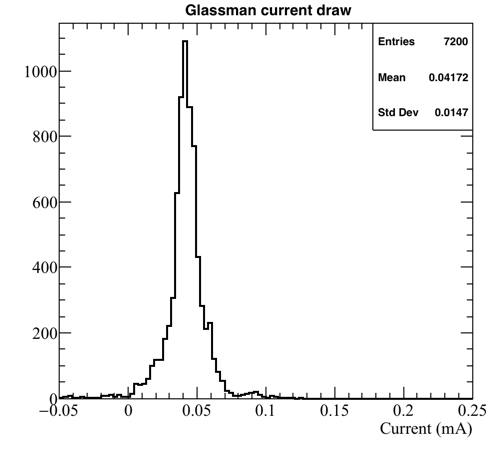
\includegraphics[width=3in]{images/glassman_current_20160525-30.png}
\caption{Current reading from the glassman between May 5th and May 10th 2016 (typical Run2 conditions).}
\label{fig:currentMeasurement}
\end{minipage}
\end{figure}




\subsection{E field using cathode-anode piercing tracks}\label{sec:CAMethode}
\subsection{E field using Michel electron sample}\label{sec:michelEl}
